\documentclass[10pt,onecolumn]{IEEEtran}

\usepackage[T1]{fontenc}
\usepackage{lmodern}
\usepackage{amsmath}
\usepackage{booktabs}
\usepackage{float}
\usepackage{graphicx}
\usepackage{microtype}
\usepackage{tabularx}
\usepackage{xcolor}
\usepackage[hidelinks]{hyperref}
\usepackage{url}

\hypersetup{
  pdftitle={Initial Technical Explanation and Preliminary Figures for Vision-Only Leader-Follower Coordination},
  pdfauthor={Neeraj Kumar Kanchani},
  pdfsubject={EE 616 technical concept and preliminary toy-model evidence},
  pdfkeywords={leader-follower robots, warehouse robotics, monocular vision, ROS 2, Gazebo}
}

\graphicspath{{../technical_explanation_report/figures/}}
\renewcommand{\arraystretch}{1.15}
\newcolumntype{Y}{>{\raggedright\arraybackslash}X}

\title{Initial Technical Explanation and Preliminary Figures\\
for Vision-Only Leader-Follower Coordination}

\author{Neeraj Kumar Kanchani\\
EE 616-57, Section 9189, Four Credits\\
Faculty Reviewer: Professor Masudul Imtiaz\\
September 18, 2026}

\begin{document}
\maketitle

\begin{abstract}
I propose a vision-only leader-follower system for warehouse material delivery.
The leader follows a route, and each follower observes the robot directly ahead with a forward RGB camera.
The follower estimates relative range and bearing, combines the measurement with local wheel odometry, and uses bounded control to maintain a requested gap.
This report explains the proposed system and presents results from a deterministic two-dimensional toy model.
The toy results confirm the experiment structure, logging, and basic control behavior under simplified conditions.
They do not validate ROS 2 timing, Gazebo physics, image detection, physical robots, or production safety.
I request feedback on the technical structure and on the plan to validate one leader-follower pair before adding more followers.
\end{abstract}

\begin{IEEEkeywords}
leader-follower robots, warehouse robotics, monocular vision, formation control, ROS 2, Gazebo
\end{IEEEkeywords}

\section{Technical Purpose and Review Request}

The application is a flexible material-delivery convoy for warehouse and manufacturing aisles.
The leader owns the route.
Each follower is an independently driven cart that tracks the robot directly ahead.
Follower 1 tracks the leader, Follower 2 tracks Follower 1, and later followers use the same pattern.

My main technical question is:

\begin{quote}
How accurately and reliably can a follower maintain a requested gap using a forward RGB camera and local wheel odometry during changes in range, heading, speed, turns, and short visual occlusions?
\end{quote}

The current evidence comes from a deterministic Python toy model.
It includes a camera-like range and bearing calculation, a state estimator, bounded control, three recovery states, synchronized logging, automated tests, and repeatable plots.
The model is useful for checking the experiment design before a more expensive simulator is introduced.

The main limitation is clear.
The model does not include rendered camera images, learned detection, robot dynamics, wheel slip, ROS 2 communication, or Gazebo physics.
It also does not provide evidence of industrial safety.

I am asking for feedback on three points.
First, is one leader and one follower the correct minimum experiment?
Second, is a known visual target acceptable for the first camera measurement study?
Third, are the proposed error, timing, and resource measurements sufficient before I extend the convoy?

\section{Verified Project State}

Table~\ref{tab:verified} lists the current verified condition.
The values are taken from the saved JSON and CSV evidence files in the project repository.

\begin{table}[H]
\caption{Verified Evidence and Its Meaning}
\label{tab:verified}
\centering
\small
\begin{tabularx}{\linewidth}{@{}p{0.20\linewidth}p{0.32\linewidth}Y@{}}
\toprule
Item & Verified condition & Meaning \\
\midrule
Automated tests & Seven tests pass & The recorded toy functions are deterministic and finite. \\
Pair experiment & 32 trials across four scenarios and eight seeds & The experiment can be repeated under the same simplified assumptions. \\
Warehouse run & One leader, three followers, 86 simulated seconds, and seven completed route segments & The planned chain structure and logging work in the toy maze. \\
Collision record & Zero collision samples in the toy collision check & No collision was recorded by the center-and-radius model. This is not a safety result. \\
ROS 2 and Gazebo & A complete working stack has not been verified & No ROS 2 or Gazebo performance result is claimed. \\
\bottomrule
\end{tabularx}
\end{table}

\section{System Topology and Experimental Boundary}

Figure~\ref{fig:topology} shows the proposed system.
Each follower contains the same perception, estimation, supervision, and control pipeline.
Each robot will use a separate ROS 2 namespace so that topics and parameters remain isolated.
ROS 2 topics are intended for continuous sensor and state streams in this design~\cite{ros2_interfaces}.

\begin{figure}[!t]
\centering
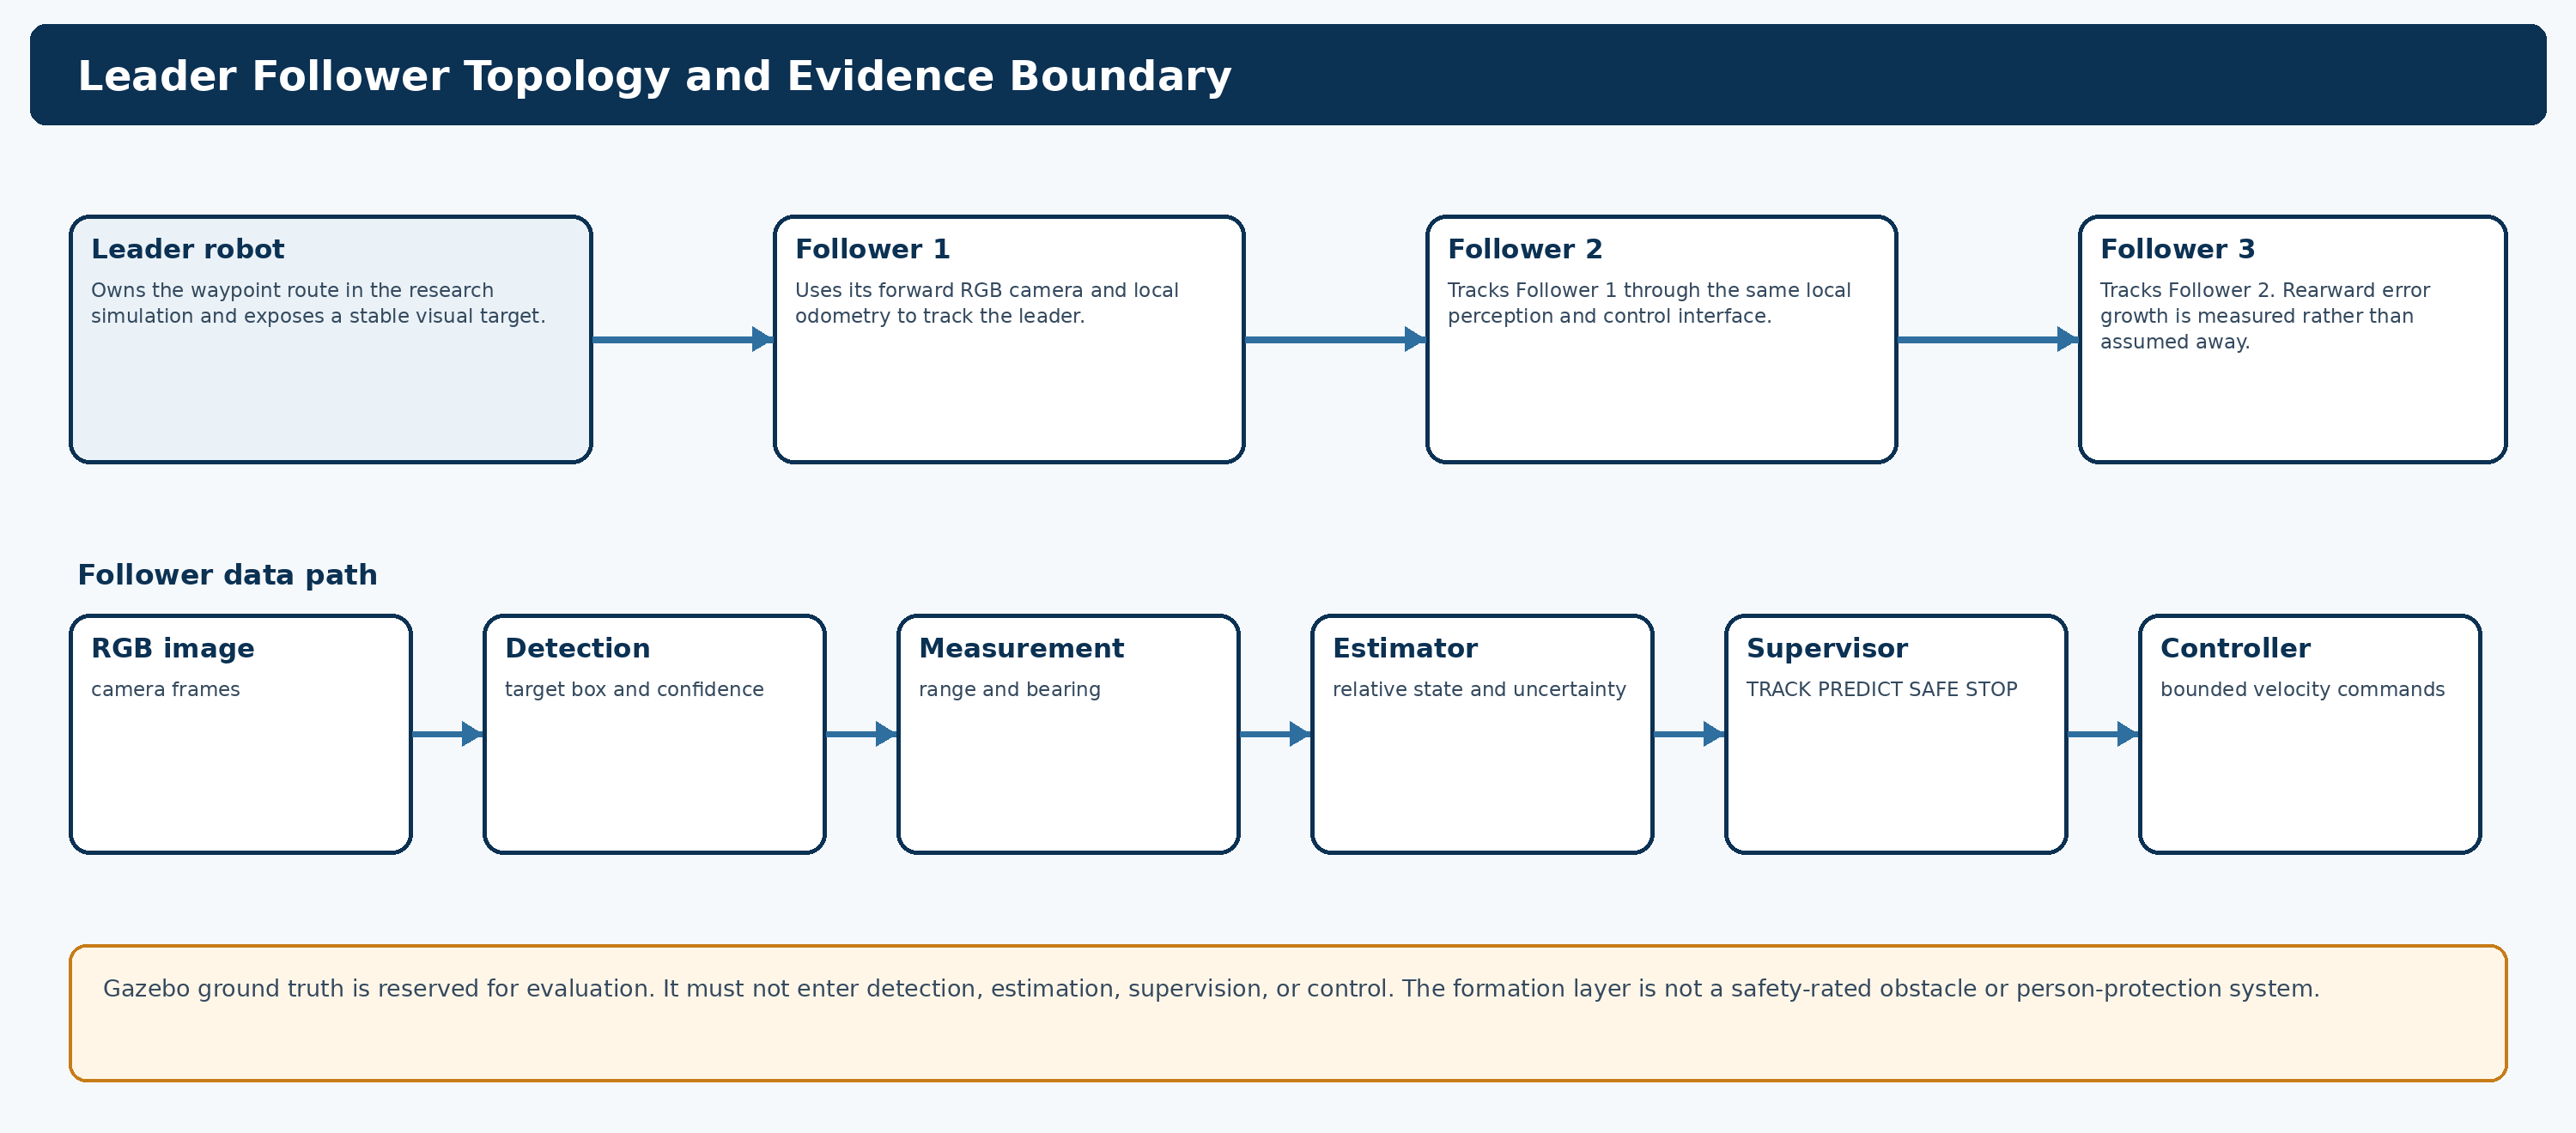
\includegraphics[width=0.96\linewidth]{figure_1_system_topology.png}
\caption{Proposed predecessor-following topology. Gazebo ground truth is outside the control path and is reserved for evaluation.}
\label{fig:topology}
\end{figure}

Predecessor following reduces the viewing requirement for rear robots.
A rear follower does not need to see the leader through the complete convoy.
However, local errors can grow toward the rear.
The project will therefore validate one pair first and add later followers one at a time.

Gazebo ground truth may be recorded by the evaluator.
It must not enter target detection, state estimation, supervision, or control.
This separation prevents the controller from using information that a camera-based physical robot would not have.

\section{Camera-Only Range and Bearing Measurement}

The toy camera model uses a known target height.
Let $H$ be the real target height, $h$ the detected image height, $f$ the camera focal length in pixels, $u$ the horizontal center of the detected box, and $c_x$ the horizontal camera principal point.
The model estimates range $r$ and bearing $\theta$ as

\begin{equation}
r = \frac{fH}{h},
\end{equation}

\begin{equation}
\theta = \tan^{-1}\left(\frac{u-c_x}{f}\right).
\end{equation}

Figure~\ref{fig:camera} illustrates these measurements.
Pixel noise is added before the range and bearing calculations.
A later image detector would provide the target box and confidence value, but the geometry can be tested separately.

\begin{figure}[!t]
\centering
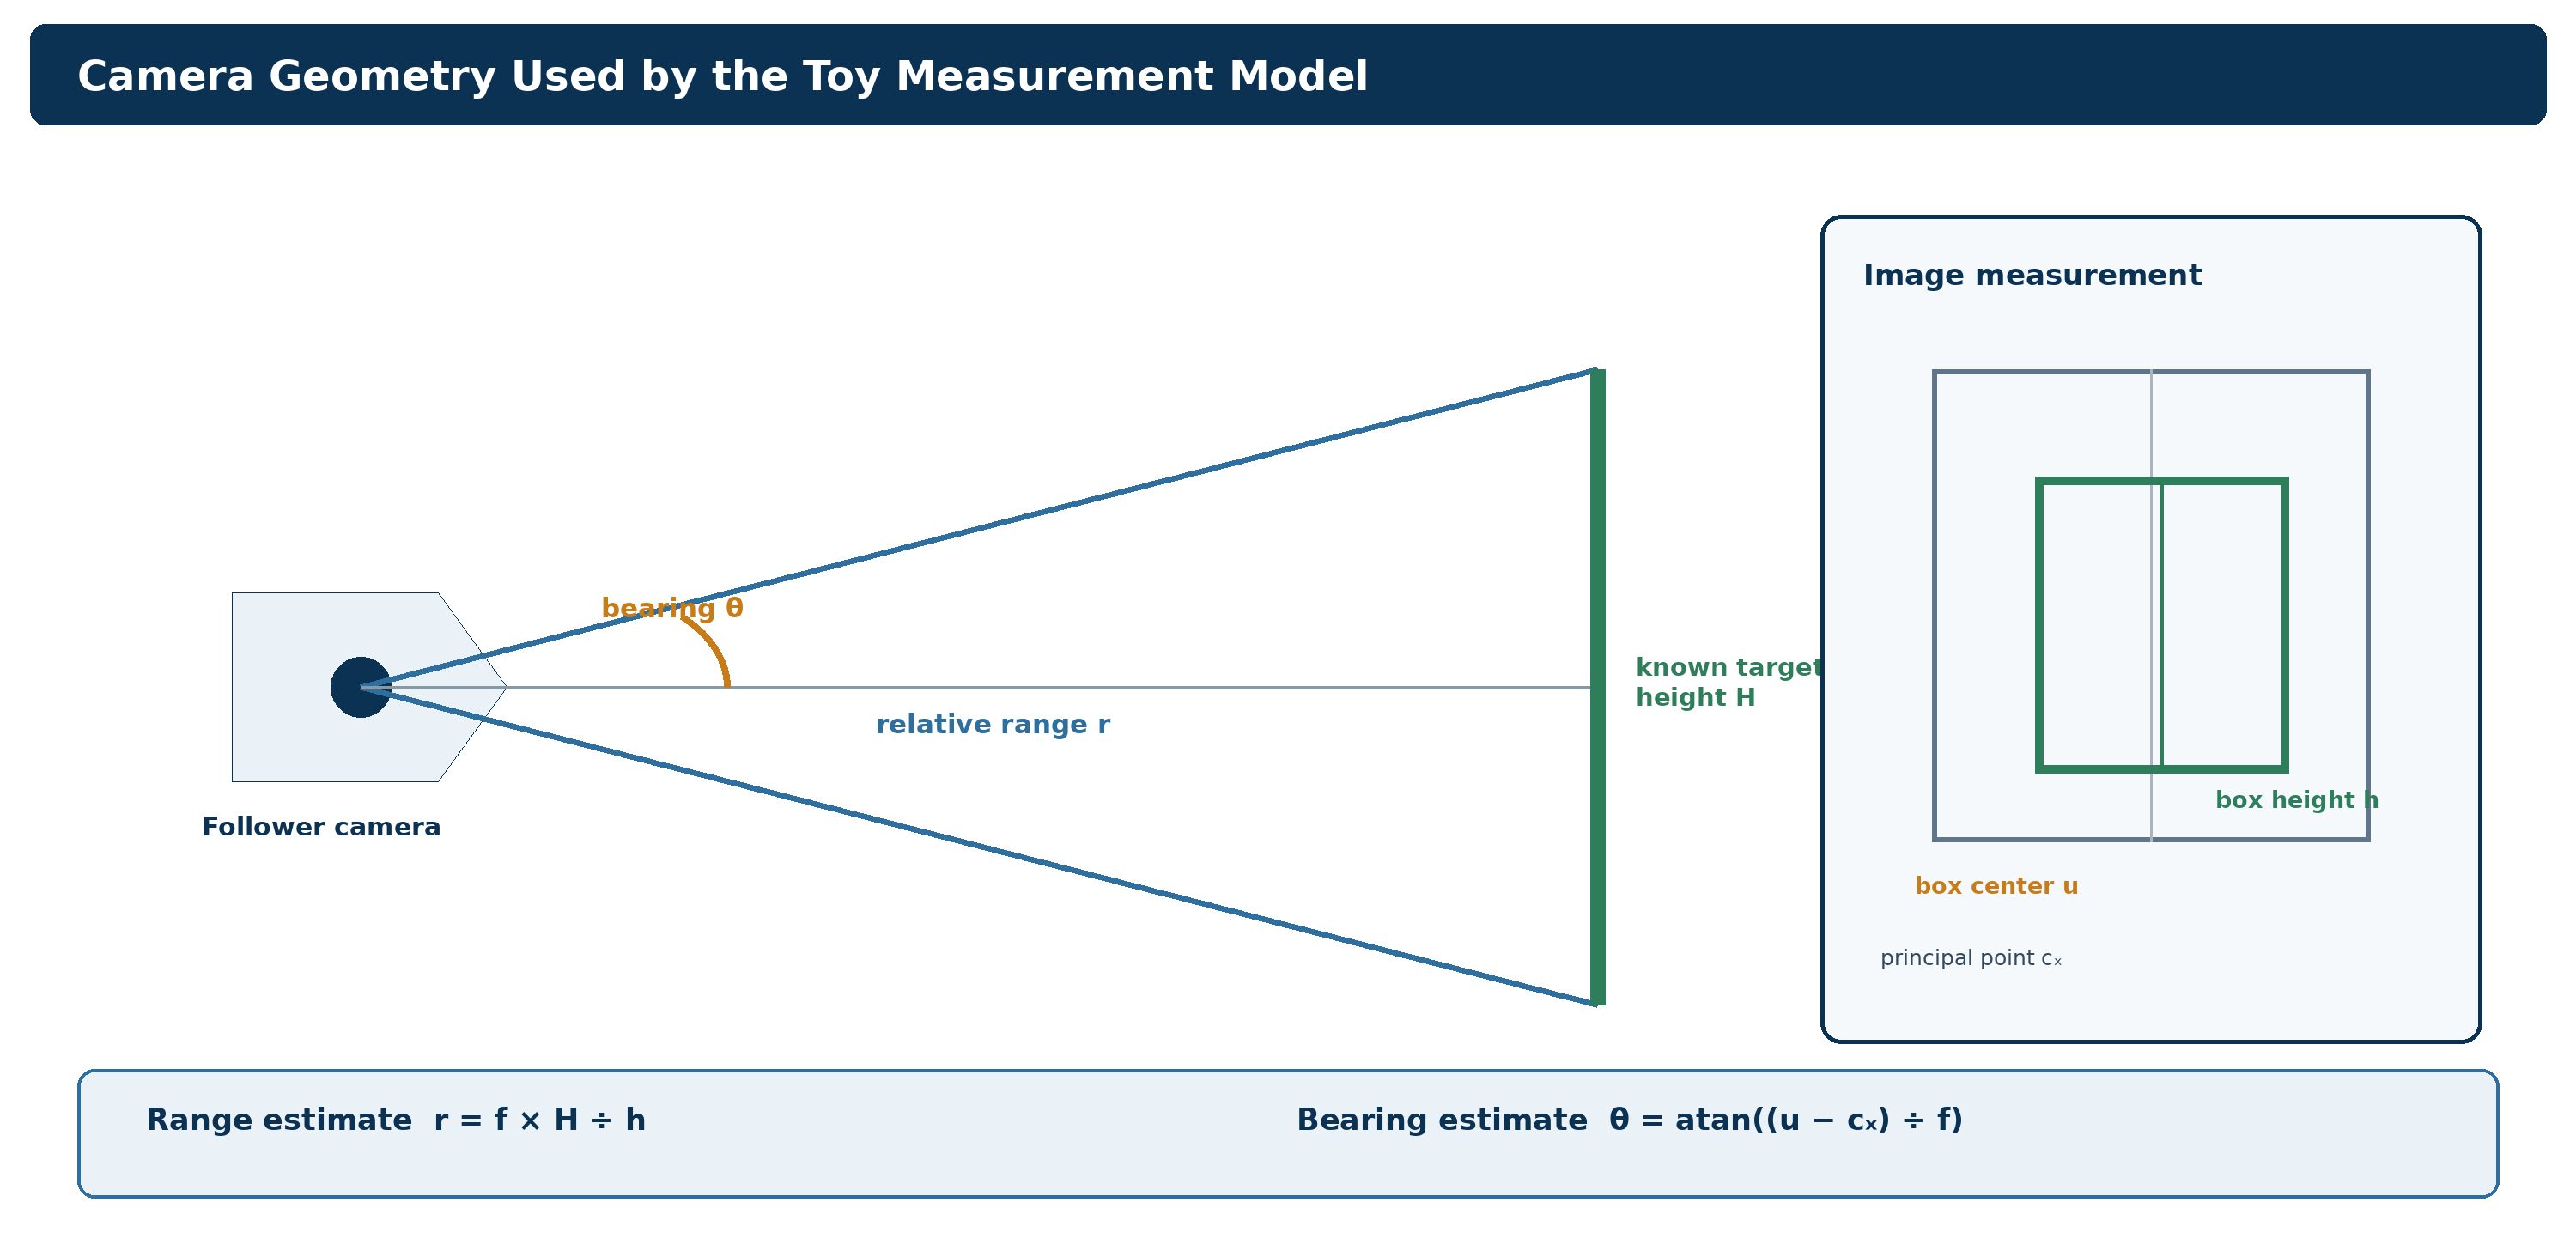
\includegraphics[width=0.96\linewidth]{figure_2_camera_geometry.png}
\caption{Monocular range and bearing calculation used by the toy camera model.}
\label{fig:camera}
\end{figure}

This method has known limits.
A small, clipped, tilted, or partly hidden target can produce an incorrect height measurement.
The first Gazebo camera experiment should therefore change target range, horizontal position, heading, lighting, and visibility.
Gazebo Harmonic provides simulated sensors, but the existence of a camera sensor does not prove measurement accuracy~\cite{gazebo_sensors}.
Accuracy must be measured against synchronized evaluation data.

\section{Estimation, Control, and Recovery}

The current filter estimates the predecessor's two-dimensional position and velocity.
It predicts the state every 0.02 seconds and applies a correction when a camera sample is available.
The toy model transforms each camera measurement into the world frame by using an ideal follower pose.
This ideal pose is a major simplification.
The ROS 2 implementation must instead use local wheel odometry and record covariance, measurement time, and state age.

The controller combines estimated forward target speed with proportional range and bearing terms.
It limits the maximum linear and angular commands.
The supervisor has three states:

\begin{itemize}
    \item \textbf{TRACK}: use a recent valid camera measurement and apply bounded control;
    \item \textbf{PREDICT}: continue a short estimator prediction while the target is temporarily unavailable;
    \item \textbf{SAFE STOP}: command zero linear and angular velocity when the estimate is unavailable or too old.
\end{itemize}

Figure~\ref{fig:supervisor} shows this sequence.
These states define predictable software behavior during target loss.
They do not establish a certified stopping distance or a safety-rated control system.

\begin{figure}[!t]
\centering
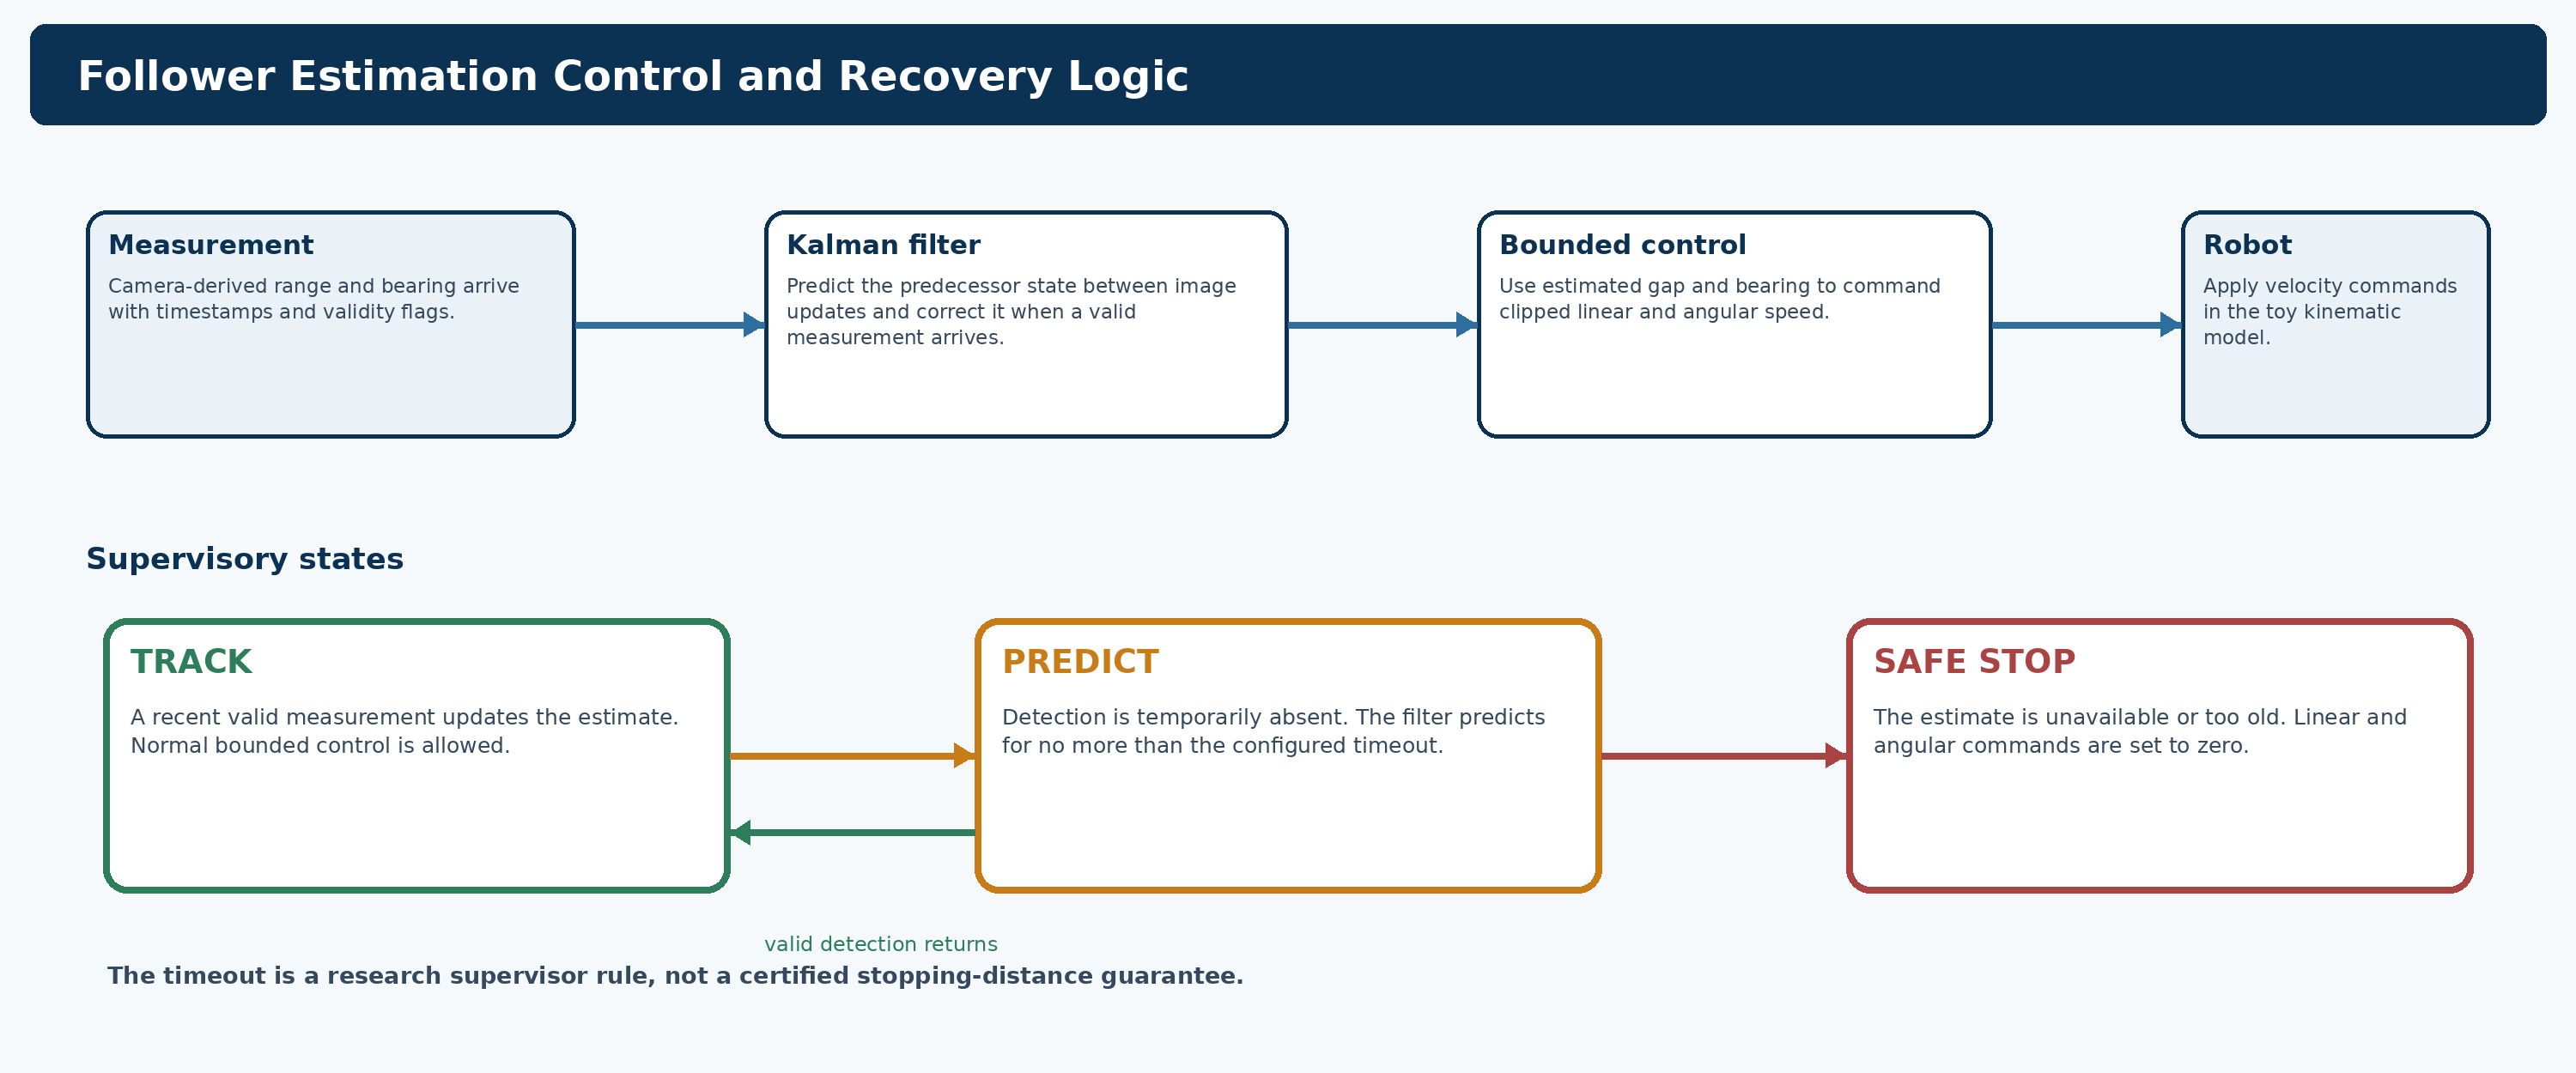
\includegraphics[width=0.96\linewidth]{figure_3_state_supervisor.png}
\caption{Estimation, bounded control, and the TRACK, PREDICT, and SAFE STOP supervisor.}
\label{fig:supervisor}
\end{figure}

\section{Preliminary Toy Evidence}

The single-pair baseline contains 32 trials.
The scenarios are straight motion, an S-curve, a constant-radius turn, and a forced visual occlusion.
Eight recorded random seeds are used for each scenario.

Across those trials, the median synthetic range root-mean-square error (RMSE) was 0.011 m.
The median bearing mean absolute error was 0.104 degrees.
The median formation RMSE was 0.009 m.
The median reacquisition time after the forced occlusion was 0.030 s.
The toy collision check recorded zero collision samples.

The warehouse demonstration used one leader and three followers for 86 simulated seconds.
It completed seven route segments through a six-shelf maze.
The toy collision check again recorded zero collision samples.
The spacing RMSE was 0.140 m for Follower 1, 0.164 m for Follower 2, and 0.200 m for Follower 3.

Figure~\ref{fig:results} shows the recorded trajectories and spacing errors.
The increasing error toward the rear is important.
It supports measuring error propagation and corner behavior when followers are later added to the validated pair.
It does not show that the current convoy is ready for a physical warehouse.

\begin{figure}[!t]
\centering
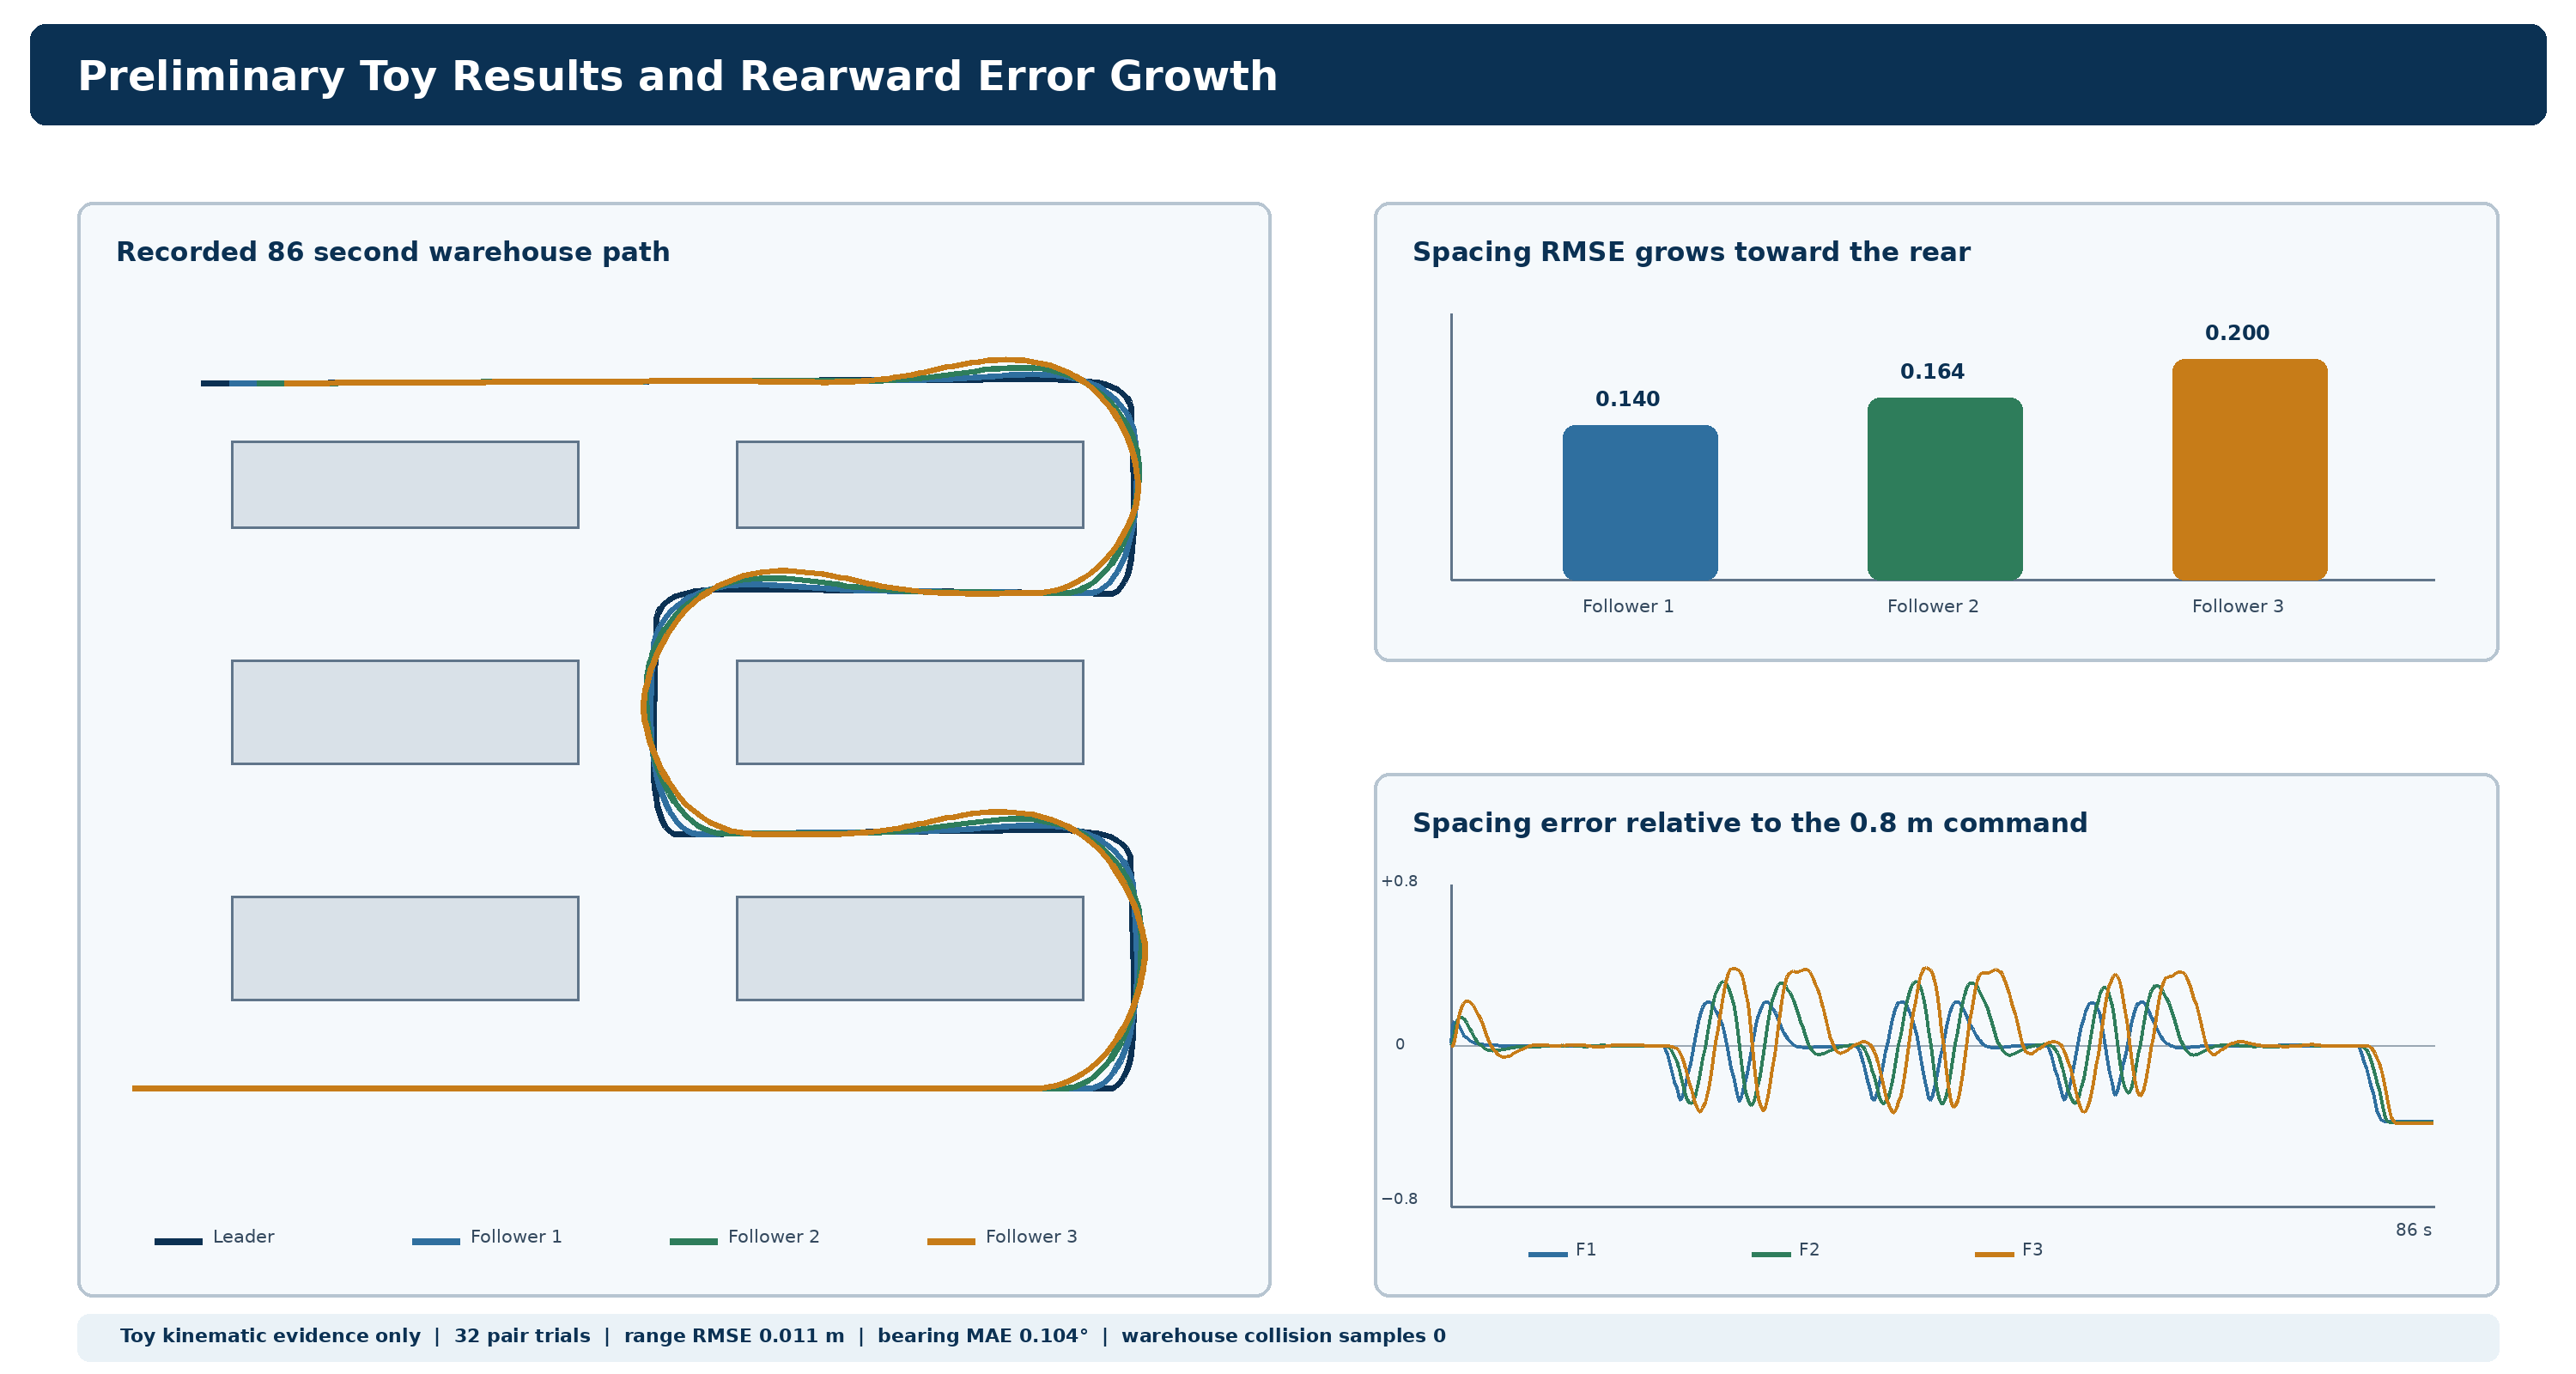
\includegraphics[width=0.96\linewidth]{figure_4_preliminary_results.png}
\caption{Recorded toy trajectories, spacing error, and error growth toward the rear of the convoy.}
\label{fig:results}
\end{figure}

\section{What the Evidence Does Not Prove}

Table~\ref{tab:limits} separates the missing conditions from the evidence required later.

\begin{table}[H]
\caption{Current Limitations and Required Later Evidence}
\label{tab:limits}
\centering
\small
\begin{tabularx}{\linewidth}{@{}p{0.22\linewidth}p{0.34\linewidth}Y@{}}
\toprule
Missing condition & Why it matters & Required later evidence \\
\midrule
Rendered camera frames and detection & The toy model generates target boxes directly. It omits image artifacts, false detections, and confidence changes. & Gazebo images, labeled detections, missed detections, confidence, and error against evaluation-only ground truth. \\
Robot physics and odometry error & The model omits wheel slip, actuator delay, contact dynamics, and odometry drift. & Gazebo motion logs and controlled disturbances after the measurement gate. \\
ROS 2 timing and namespaces & The current code does not test middleware timing, queues, quality of service, or namespace isolation. & Timestamp audits, topic graphs, launch tests, and dropped-frame measurements. \\
Inference resources & Synthetic geometry does not measure detector latency or GPU memory. & An ordinary FP32 baseline followed by optimization only when measured results justify it. \\
Industrial safety & A formation controller is not a safety-rated person or obstacle protection system. & Independent safety architecture, verified stopping behavior, site risk assessment, commissioning, and standards work. \\
\bottomrule
\end{tabularx}
\end{table}

ISO 3691-4:2023 addresses safety requirements and verification for driverless industrial trucks and their systems~\cite{iso3691}.
The toy model, Gazebo work, and later simulation results will not be presented as compliance evidence.
Formation coordination will remain separate from independent safety functions.

\section{Recommended Next Technical Gate}

I recommend validating the software environment before building the camera experiment.
The environment gate should record the installed ROS 2 and Gazebo versions, shell setup, a namespaced publisher-subscriber test, a small Gazebo camera world, CPU and GPU availability, and repeatable setup instructions.
Gazebo Harmonic is a long-term release and lists Ubuntu Noble on amd64 as a supported platform~\cite{gazebo_install}.

After the environment gate passes, I recommend a measurement-only camera experiment.
The follower camera should observe a known target over a controlled pose grid.
Estimated range and bearing should be compared with synchronized Gazebo ground truth used only by the evaluator.
The controller should remain outside that experiment.
This keeps a camera measurement error from being hidden by closed-loop motion.

\section{Questions for Faculty Review}

\begin{enumerate}
    \item Is the one-pair camera measurement experiment an appropriate minimum scientific unit before closed-loop control?
    \item Is a known visual target acceptable for the first Gazebo baseline before a learned detector is introduced?
    \item Are range error, bearing error, timing, missed detections, and resource use sufficient measurements for the first camera review?
    \item Should the final demonstration target one leader and three followers only if the pair and incremental-chain tests pass?
\end{enumerate}

\section{Evidence Files}

The numerical results in this report come from the following project files:

\begin{itemize}
    \item \texttt{work/toy\_simulation/results/summary.json};
    \item \texttt{work/toy\_simulation/results/trial\_metrics.csv};
    \item \texttt{work/toy\_simulation/warehouse\_results/warehouse\_multi\_summary.json};
    \item \texttt{work/toy\_simulation/warehouse\_results/warehouse\_multi\_timeseries.csv}.
\end{itemize}

The implementation is stored under \path{work/toy_simulation/src}.
The automated tests are stored under \path{work/toy_simulation/tests}.

\bibliographystyle{IEEEtran}
\bibliography{references}

\end{document}
